\section{Mathematical Preliminaries}

In this section we recall some mathematical notions
we shall need to discuss the last two algorithms, 
Newton-Grassmann and Differential-Geometric Newton methods.

\subsection{Newton method}

Let us recall some basic facts about ordinary Newton method. The minimization problem for 
a smooth function is usually reduced to finding zero of the gradient, 
so we shall discuss solving system of equations
$f(x) = 0$, $f \colon \R^n \to \R^n$.

 Geometrically the idea of the method in one-dimensional case is 
to move along the tangent lines to the graph of $f$. Analytically this is expressed by the following iterative formula:
\begin{equation}
 x_{n+1} = x_n - \frac{f(x_n) }{ f'(x_{n})}. 
\end{equation}


%\begin{figure}
%        \centering
%                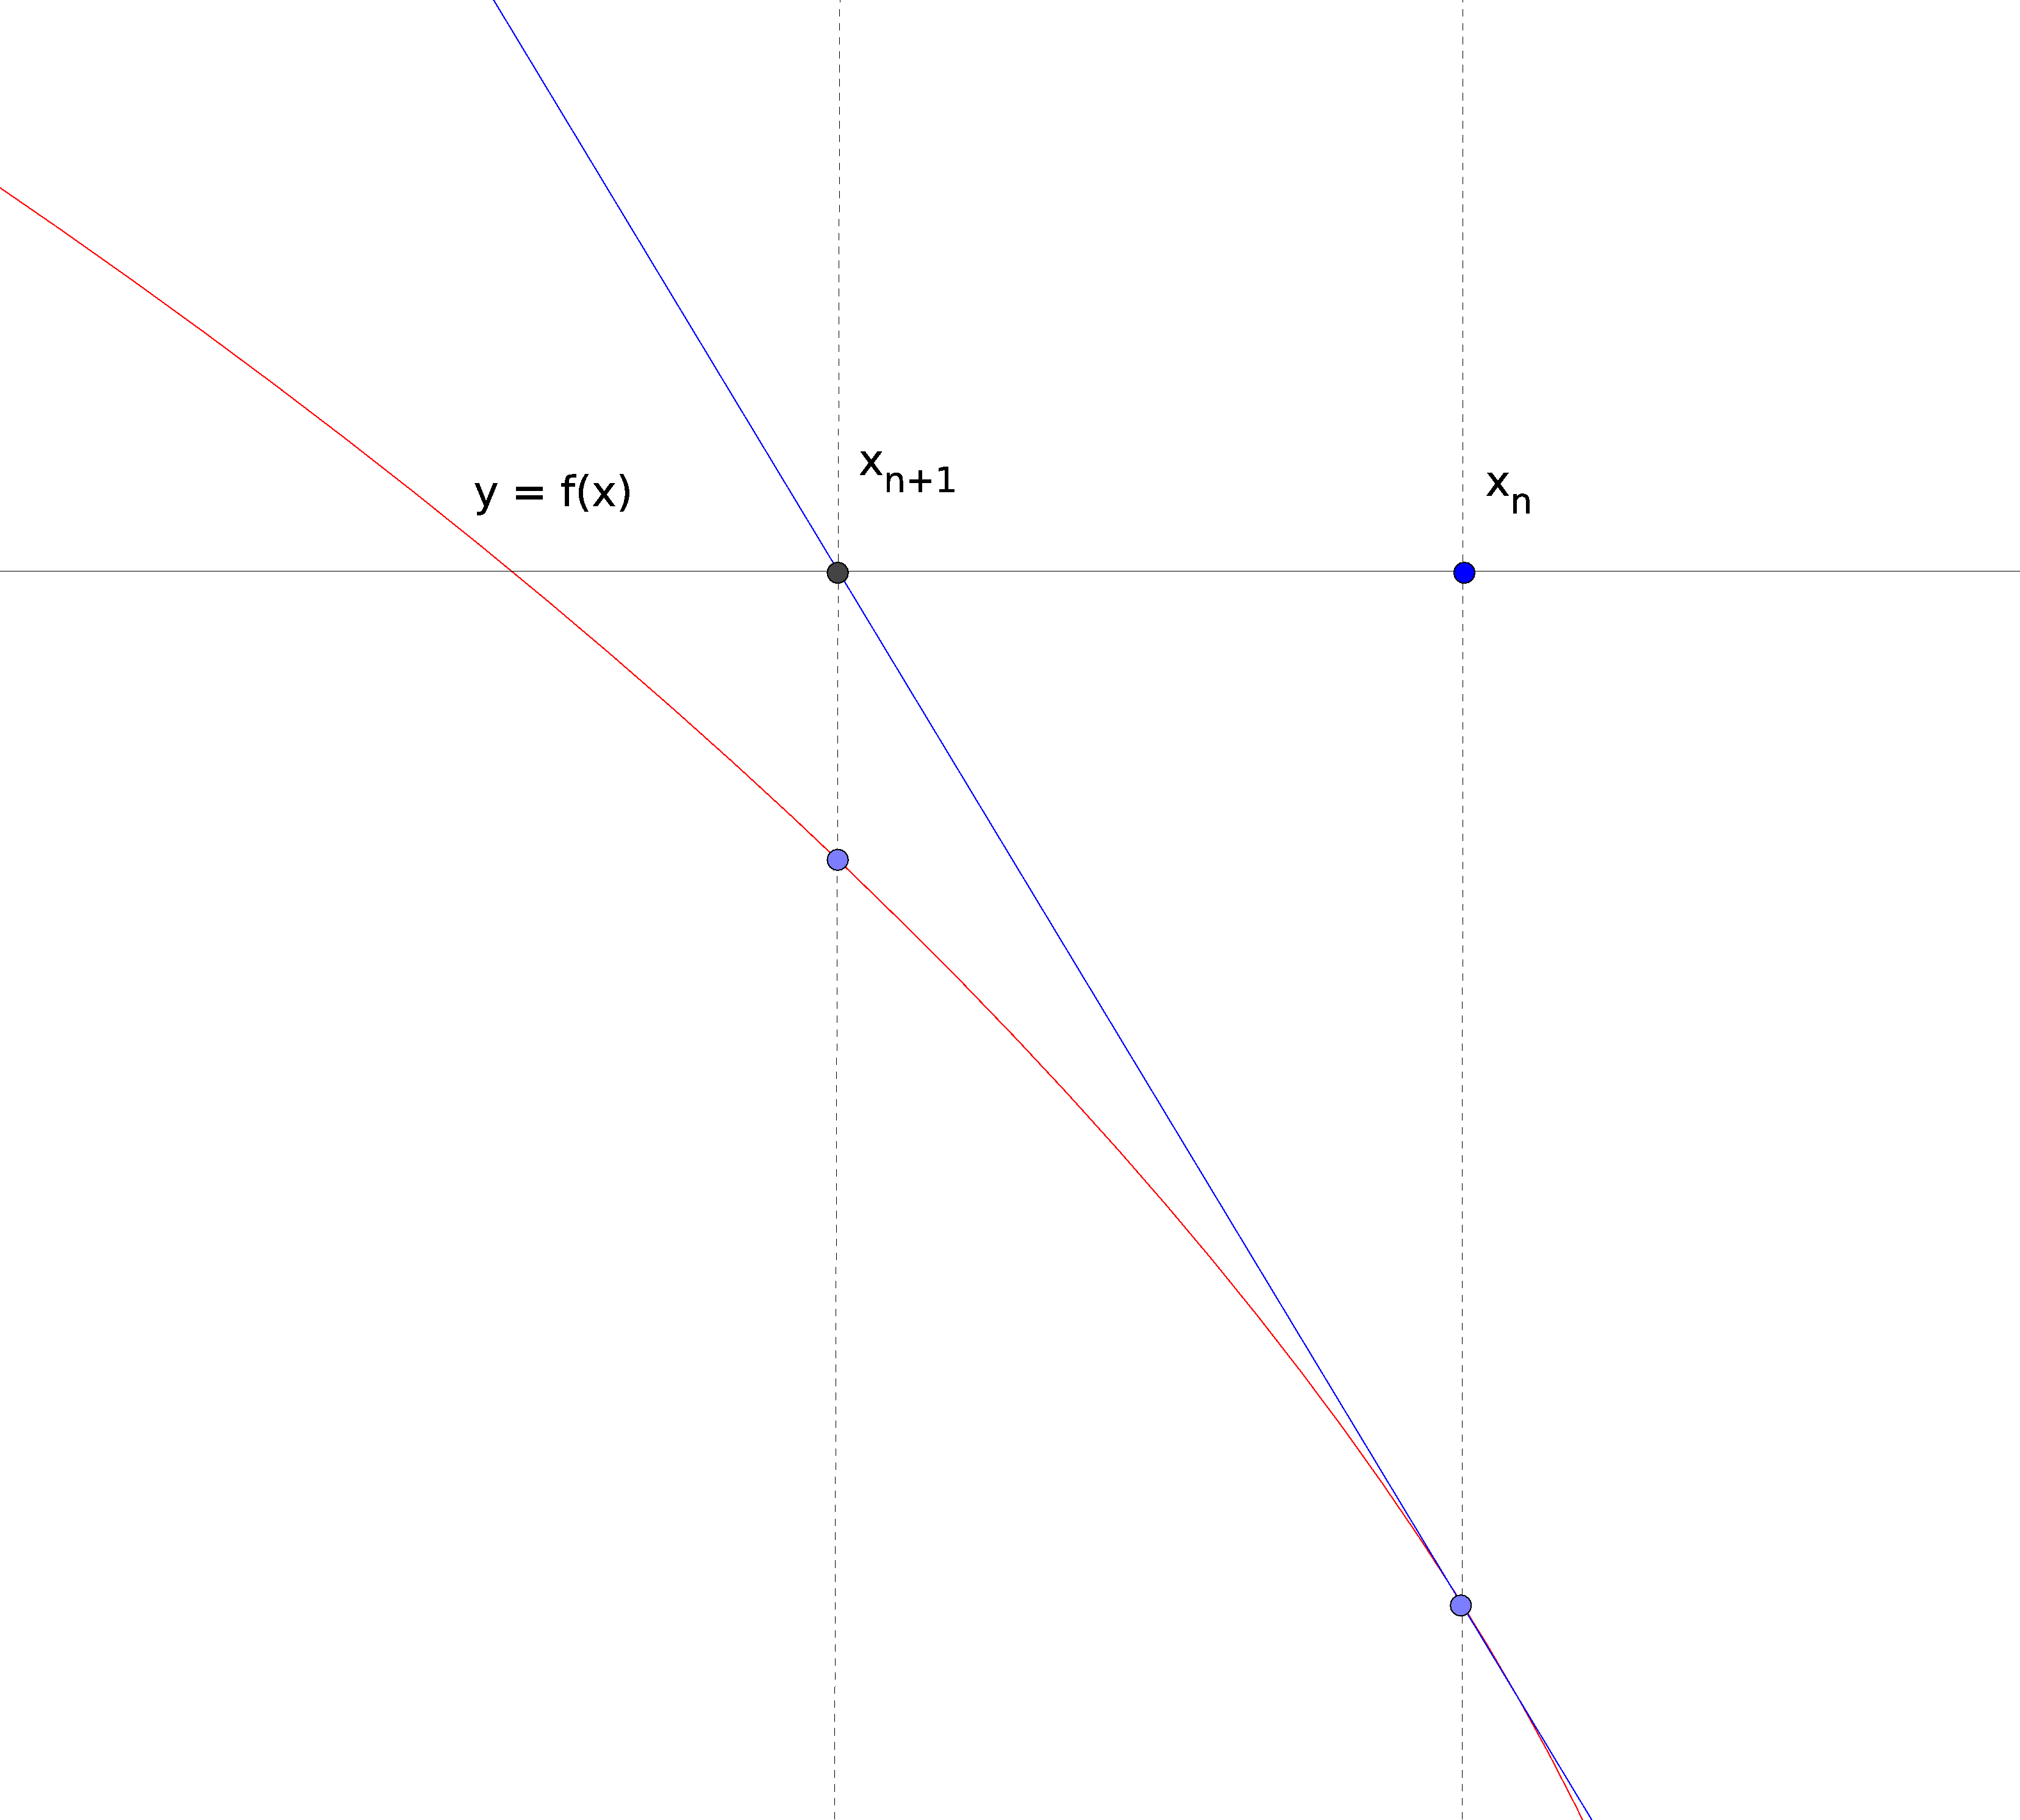
\includegraphics[width=8cm]{images/newton-image1.png}
%        \caption{Newton's method illustration}
%        \label{fig:newt_method_tangents}
%\end{figure}

The method is known to be very fast-convergent (providing that the initial value $x_0$ is close enough to a root).
In multivariate case the formula is
\begin{equation}
 x_{n+1} = x_n - ((Df)(x_n))^{-1} ( f(x_n) ).
\end{equation}
Here $(Df)(x_n)$ denotes the Jacobi matrix of the mapping $f$. In practice, instead of finding
the inverse of this matrix and then applying it to the vector $f(x_n)$, it is 
easier to solve the linear system $(Df)(x_n) y = f(x_n) $, but still this step is computationally expensive,
especially if the number of variables is high.


If we use this method to minimize $F$ by finding the zero of $\nabla F$, then
we can also interpret this method in terms of $F$. If we approximate $F$
with its Taylor expansion of degree $2$, then in a neighbourhood 
of a non-degenerate extremum point the level sets will be ellipses.
The gradient is known to be orthogonal to level set, so, if we use gradient descent,
we may come to the optimum quite slowly, if the ellipses are very elongated.
The Newton's method involves inverting of $D (\nabla F)$, that is, inverting 
the Hessian of $F$, which is exactly the quadratic part of the Taylor expansion.
By inverting it we essentially transform our problem to a coordinate system in which
the level sets are circular and this allows us to move to the optimum much faster (see Figure \ref{fig:newt_grad_comp}).

\begin{figure}
        \centering
                
\includegraphics[width=4cm]{images/newton_vs_grad_desc.jpg}
        \caption{Newton's method illustration}
        \label{fig:newt_grad_comp}
\end{figure}


However, Newton method is known to behave poorly, if the root is not isolated.
This is exactly the situation we have in Tucker2 decomposition, where the objective function
does not change, if factor matrices are multiplied by any orthogonal matrices. 
%The geometric interpretation of this operation is that we choose another orthonormal basis in the same subspace.
There are orthogonal matrices approximately close to the identity matrix, so the zeros
of the gradient w.r.t. entries of $F_2$, $F_3$ are not isolated. In order to apply Newton method
we need to work in more geometric terms, and we start by brief informal description of the notions
that are necessary, namely: smooth manifold, tangent space, differential of a mapping between two smooth manifolds,
Riemannian metric, geodesic.
We are not going to give 
rigorous mathematical definitions, otherwise it would be necessary
to reproduce a significant part of several mathematical textbooks.
Instead we give a very informal description, which should be sufficient
to understand the intuition behind the two remaining methods.


\subsection{Some notions from differential geometry}
\subsubsection{Smooth manifolds}
A smooth manifold of dimension $n$ is a space which locally 
looks like $\R^n$. 
This means that in a neighbourhood of each point we have a local coordinate system $(x_1(\cdot), \dots,  x_n(\cdot))$.
Point $p$ of a manifold $M$ in this system is described by 
\begin{equation}
p \mapsto (x_1(p), \dots, x_n(p)) \in \R^n. 
\end{equation}
Usually these coordinate systems  cover only a part of the manifold, but each point belongs to the domain
of at least one of them.
If the domains of two coordinate systems $(x_1(\cdot), \dots, x_n(\cdot))$
and $(y_1(\cdot), \dots, y_n(\cdot))$ intersect, then we have transition functions
\begin{equation}
(x_1, \dots, x_m) \mapsto (y_1, \dots, y_n) \mbox{ if } \exists p : x_i(p) = x_i \mbox{ and } y_i(p) = y_i \mbox{ for all } i.
\end{equation}
These functions must be differentiable (this is a part of the definition of smooth manifold).
This approach to manifolds does not require them to be a subset of 
any ambient Euclidean space $\mathbb{R}^N$. There is Whitney's embedding theorem 
that states that any manifold can be embedded into $\mathbb{R}^N$
for some $N$. However, sometimes there is no good or natural way to choose this embedding.

\begin{enumerate}
    \item $\R^n$ is a manifold (the identity mapping is a coordinate system that
        covers the whole space). Since every finite-dimensional vector space is 
        isomorphic to $\R^n$, vector spaces are also manifolds. In particular,
        the space of $m \times n$ matrices is a manifold isomorphic to $\R^{mn}$.
    \item If $M$ is a manifold, then every open subset of $M$ is also a manifold.
        In particular, the set of $m \times n$ matrices with some fixed rank $k$
        is a manifold. We shall need the set $\R^{n \times n}_{*}$ of non-singular $n \times n$ matrices,
        which is a manifold by this remark.
    \item If $M$ is a smooth manifold and there is an equivalence relation $\sim$ on $M$,
        then, under some conditions, the set of equivalence classes $M / \sim$ is 
        also a manifold (\textit{quotient manifold theorem}, see J. M. Lee \cite{lee_manifolds}, Theorem 9.16).
    \item If $M$ and $N$ are smooth manifolds, then $M \times N$ is a smooth
        manifold.
\end{enumerate}


\subsubsection{Tangent Space}

Let $p$ be an arbitrary point of a smooth manifold $M$. The tangent space at $p$
is a vector space of the same dimension as $M$ and it is denoted by $T_pM$.
Suppose that for each point $p \in M$ we choose one vector $X_p \in T_pM$. 
This gives us a mapping $X: M \to \cup_{p \in M} T_pM$ called a
\textit{vector field on $M$}.


The notion of a tangent space is intuitively clear if we think about something like a sphere.
However, if $M$ is an open subset of $\R^n$, the tangent space at each point
is also $\R^n$.
\begin{equation}
    \forall p \in \R^n \quad T_p\R^n = \R^n.
\end{equation}
We shall often use this in the discussion of Newton methods, because
it allows us to treat matrix-valued functions of matrix argument $\R^{m \times n} \to \R^{m \times n}$
as vector fields on the manifold of matrices ($\R^{m \times n} \cong \R^{mn}$ as vector spaces).


\subsubsection{Differential and Gradient}

Generally speaking, the only structure that $T_pM$ has is that of a vector space, there is no
inner product and there is no correspondence between $T_pM$ and $T_qM$ for different
points $p, q \in M$. However, this structure is sufficient to define a differential
of a mapping between two smooth manifolds. Let $f : M \to N$ be a smooth
function between smooth manifolds $M$ and $N$ (this means that, if we write
$f$ in local coordinates on some part of $M$ and the corresponding part of $N$,
we get a smooth function of real arguments). The differential of $f$
at point $p \in M$ is a linear operator $(Df)_p : T_pM \to T_{f(p)}N$ which in
local coordinates is given by the Jacobi matrix. In particular,
if $f : M \to \R$ is a smooth real-valued function on $M$, its differential at point $p$,
called \textit{gradient} is a linear functional on $T_pM$,
so the gradient of a function is not a vector (element of a tangent space),
but a covector (element of an adjoint space $(T_pM)^*$).


If $f$ is a bijection between two smooth manifolds $M$ and $N$ such that
for all $p \in M$ and $q \in N$ the linear operators
$(Df)_p$ and $(D(f^{-1}))_q$ are non-singular, then $f$ is said to be a \textit{diffeomorphism}.
Manifolds $M$ and $N$ are \textit{diffeomorphic}, if there exists a diffeomorphism between them.

\subsubsection{Riemannian Metric}

If each $T_pM$ is equipped with an inner product
that changes smoothly as we move along $M$, then $M$ is said to be a Riemannian manifold.
A smooth curve on $M$ is a smooth mapping $\gamma : [a, b] \rightarrow M$.
Its differential at point $p \in (a, b)$ is a linear mapping $(D\gamma)(p) : T_p(a,b) \to T_pM$.
By the previous remark, $T_p(a, b) = T_p \R = \R$, and we can calculate $(D\gamma)_p(1) \in T_pM$.
This element of $T_pM$ is called \textit{velocity vector}, and we can calculate
its Euclidean norm using the inner product in $T_pM$. This defines a real-valued function
on $(a, b)$. By definition, the length of the curve $\gamma$ is the integral
of this function over $(a,b)$, so the Riemannian structure allows us to measure curves on $M$.


Moreover, if $T_pM$ has an inner product, then there is a natural isomorphism
between $T_pM$ and its adjoint space $(T_pM)^*$. This means that the 
gradient of a function on a Riemannian manifold can be viewed as a vector (element
of $T_pM$).


If two different points $p, q$ on a Riemannian manifold are close enough to each other,
there is a unique shortest path connecting $p$ and $q$. 
The condition of being locally shortest path is certain differential equation
and its solutions are called geodesics. If we consider $S^2$ in $\mathbb{R}^3$, 
then geodesics are arcs of large circles. This example illustrates that in general it is not true,
that two points are connected by the unique geodesics (consider North and South poles)
or that geodesic path is always the shortest: if $p$ and $q$ are close to each other,
there is a unique large circle passing through $p$ and $q$, but it gives rise to two
geodesics: the shortest path is the shorter arc of the circle, but the longer arc 
is a geodesic, too.


\subsubsection{Fiber Bundle}

In the differential-geometric Newton method
we shall need the notion of fiber bundle.
We start with two toy examples.
A cylinder $ \{ (x, y, z) \mid x^2 + y^2 = 1, 0 \leq z \leq 1 \}$
can be split into disjoint copies of $[0,1]$ (generating lines)
parameterized by the base $\mathbb{S}^1$,
so there is one instance of $[0,1]$ attached to each point of the circle.
A M\"obius band can also be split into disjoint segments
$[0,1]$ parameterized by $\mathbb{S}^1$. Locally both the cylinder
and M\"obius band are diffeomorphic to a cartesian product
of the arc of a circle and $[0,1]$. The cylinder is, of course,
diffeomorphic to the cartesian product not just locally, but globally,
but it is not the case for the M\"obius band, where the trivial
 pieces are glued together in a non-trivial way. Both these spaces
are called total spaces of fiber bundles with the base $\mathbb{S}^1$ and fiber $[0,1]$.
Another example of a fiber bundle is a torus $\mathbb{S}^1 \times \mathbb{S}^1$,
where both the base and the fiber are circles. 

In general, a fiber bundle is a triple $( \pi, E, B)$, where
$ \pi \colon E \to B$ is a surjective mapping such that:
\begin{enumerate}
    \item The inverse image $\pi^{-1}(p)$ of each point $p \in B$ is 
    diffeomorphic to some fixed manifold $F$.
    \item Every point $p \in B$ has a neighbourhood $V_p$
    such that $\pi^{-1}(V_p)$ is isomorphic to $V_p \times F$.
\end{enumerate}
    The space $E$ is a \textit{total space} of the bundle, $B$ is a \textit{base}, and $F$ is a \textit{fiber}.

Since the tangent space is a local notion, for each point $p \in E$
the tangent space at $p$ is isomorphic to a direct sum 
of the tangent space to the base $T_h$ and the tangent space to the fiber $T_v$,
\begin{equation}
    T_p E = T_h \oplus T_v
\end{equation}
If one wants to visualize a fiber bundle,
one usually thinks of the base positioned horizontally and the fibers
attached to the base in the orthogonal (that is, vertical) direction,
therefore the space $T_h$ is called a horizontal space and the space $T_v$
is called a vertical space. This is illustrated in Figure \ref{fig:torus_tangent}. Here 
the big parallel of the torus is its base, the meridians are fibers, and the vertical and
horizontal lines are $T_v$ and $T_h$, respectively.

\begin{figure}
        \centering
                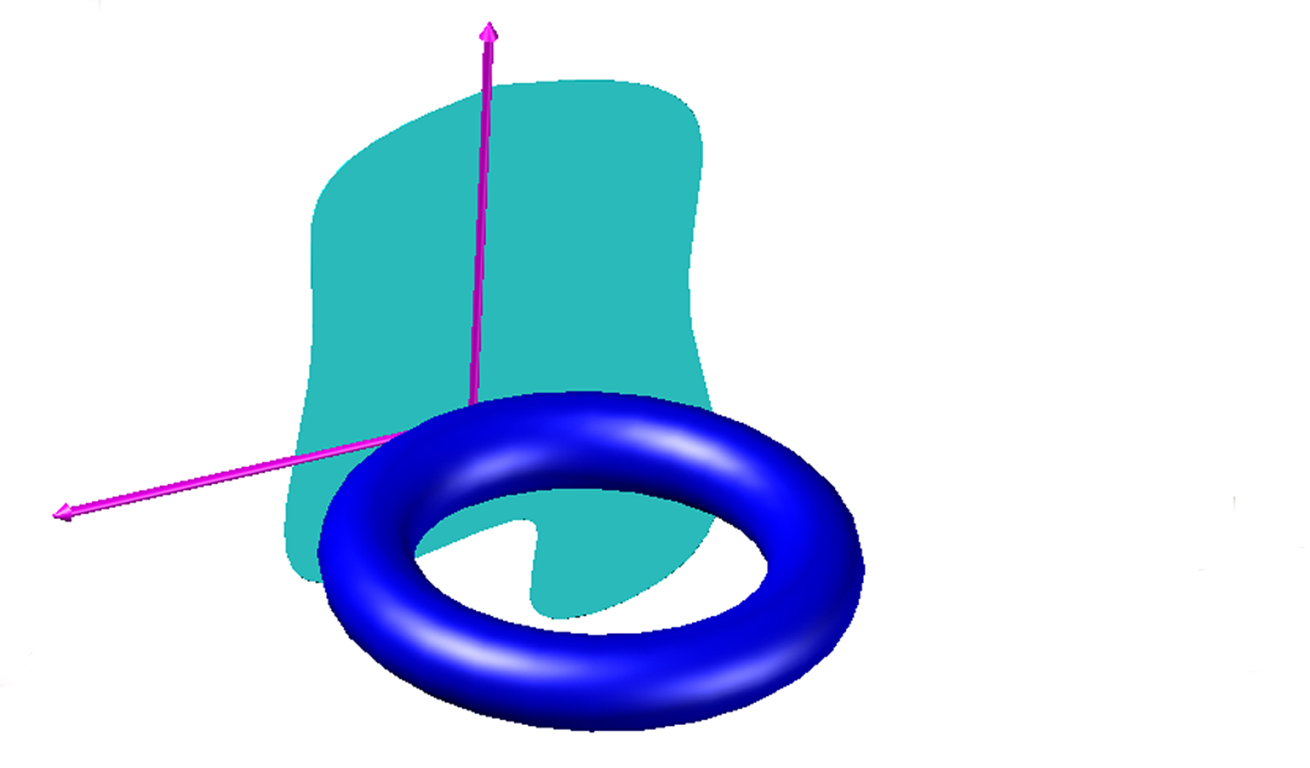
\includegraphics[width=8cm]{images/torus_tangent.jpg}
        \caption{Tangent plane to a fiber bundle.}
        \label{fig:torus_tangent}
\end{figure}

\subsubsection{Affine Connection}

The last notion we shall describe here is \textit{affine connection on a manifold}.

We say that $\nabla$ is an affine connection on a manifold $M$,
if for each vector field $X$ on $M$ we have an operator $\nabla_X$ that
maps vector fields to vector fields on $M$ and satisfies 
the following axioms:
\begin{enumerate}
    \item $\nabla_X$ is an $\R$-linear operator;
    \item (Leibniz formula) $$\nabla_X(fY) = (Xf) \cdot Y + f \nabla_X Y $$
        If $X = \sum_k b_k \frac{\partial}{\partial x_k}$ is a coordinate representation 
        of vector field $X$, then the function
        $Xf$ is defined by
        $$Xf = \sum_k b_k \frac{\partial f}{\partial x_k}$$
    \item $$ \nabla_{X + Y} = \nabla_X + \nabla_Y $$
        and
        $$ \nabla_{fX} = f \nabla_X.$$
\end{enumerate}
The field $\nabla_{X} Y$ is called the covariant derivative of $Y$ along $X$.
This operation is a generalization of differentiation in $\R^n$.
It plays a central role in differential geometry,
capturing the properties of curved spaces. In particular,
with affine connection it is possible to perform
parallel translation of a vector along a curve, so
affine connections 'connect' tangent
spaces at different points.


